\section{Planos en el Espacio}

Un plano en $\mathbb{R}^3$ se define como una superficie formada por >el conjunto de todos los puntos $(x, y, z)$ tales que la función $f(x, y, z) = ax + by + cz$ toma un valor constante $k$. 

Un plano se define de manera única si se conocen:
\begin{enumerate}
    \item Un punto de referencia $P_0(x_0, y_0, z_0)$ que pertenezca a la superficie.
    \item Un vector no nulo $\vec{n} = (a, b, c)$ que sea perpendicular a la superficie en todos sus puntos, denominado \textbf{vector normal}.
\end{enumerate}

\begin{center}
\shorthandoff{>}
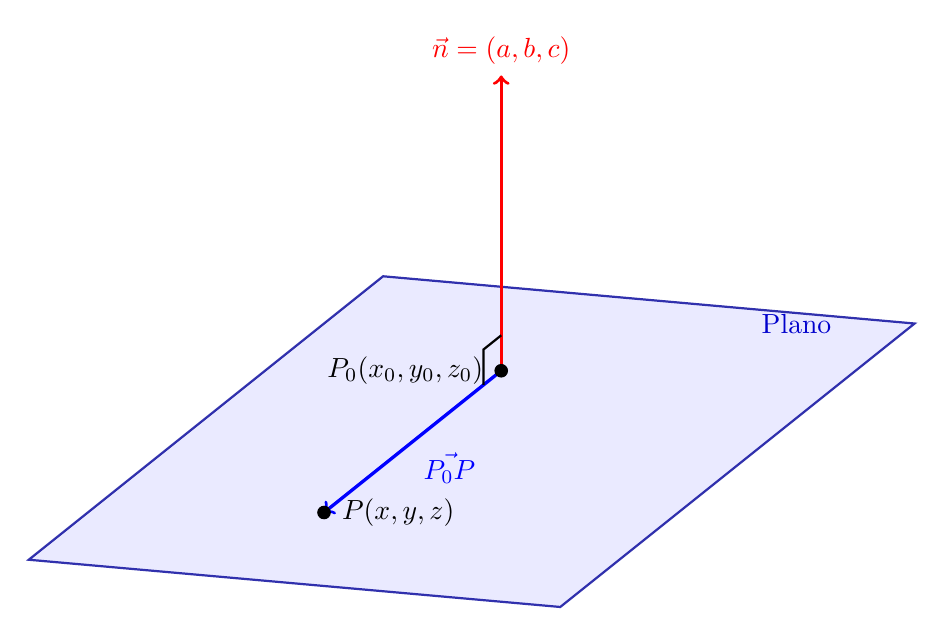
\begin{tikzpicture}[x={(-0.5cm,-0.4cm)}, y={(1cm,0cm)}, z={(0cm,1cm)}, scale=1.5]
    % Dibujo del plano (con un poco de transparencia para estética 3D)
    \filldraw[fill=blue!10!white, draw=blue!60!black, thick, opacity=0.8] 
        (-2,-2,0) -- (4,-2,0) -- (5,3,0) -- (-1,3,0) -- cycle;
    
    % Coordenadas
    \coordinate (P0) at (0,0,0);
    \coordinate (P) at (3,0,0);
    \coordinate (N) at (0,0,2.5);
    
    % Vector Normal
    \draw[->, very thick, red] (P0) -- (N) node[above] {$\vec{n} = (a,b,c)$};
    
    % Vector sobre el plano
    \draw[->, very thick, blue] (P0) -- (P) node[midway, below right] {$\vec{P_0P}$};
    
    % Indicador de perpendicularidad
    \draw[thick] (0.3,0,0) -- (0.3,0,0.3) -- (0,0,0.3);
    
    % Puntos
    \filldraw[black] (P0) circle (1.5pt) node[left=3pt] {$P_0(x_0,y_0,z_0)$};
    \filldraw[black] (P) circle (1.5pt) node[right=3pt] {$P(x,y,z)$};
    
    % Etiqueta del plano
    \node[blue!80!black] at (-1, 2, 0) {Plano};
\end{tikzpicture}
\end{center}

\subsection{Ecuación escalar y general}

Si $P(x, y, z)$ es un punto arbitrario en el plano, el vector $\vec{P_0P} = (x-x_0, y-y_0, z-z_0)$ yace en la superficie. Por definición de vector normal, $\vec{n}$ debe ser perpendicular a $\vec{P_0P}$, lo que implica que su producto punto es $0$:

$$ \vec{n} \cdot \vec{P_0P} = 0 \implies (a, b, c) \cdot (x-x_0, y-y_0, z-z_0) = 0 $$

Al desarrollar el producto punto, se obtiene la ecuación escalar del plano:

$$ a(x - x_0) + b(y - y_0) + c(z - z_0) = 0 $$

Agrupando las constantes en un solo término $d = -(ax_0 + by_0 + cz_0)$, se llega a la ecuación general del plano:
$$ ax + by + cz + d = 0 $$

\subsection{Determinación de un Plano dados Tres Puntos}

Si se conocen tres puntos no colineales $A, B$ y $C$, es posible determinar la ecuación del plano que los contiene. \\

Primero, Se definen dos vectores directores que unan los puntos dados:
    $$ \vec{u} = \vec{AB} = B - A $$
    $$ \vec{v} = \vec{AC} = C - A $$

Puesto que $\vec{u}$ y $\vec{v}$ yacen sobre el plano, su producto vectorial generará un vector perpendicular a ambos y, por lo tanto, normal al plano:
    $$ \vec{n} = \vec{u} \times \vec{v} = \begin{vmatrix} \hat{i} & \hat{j} & \hat{k} \\ u_1 & u_2 & u_3 \\ v_1 & v_2 & v_3 \end{vmatrix} = (a, b, c) $$

Con el vector normal $(a, b, c)$ y utilizando el punto $A(x_1, y_1, z_1)$ como referencia, se aplica la ecuación escalar:
    $$ a(x-x_1) + b(y-y_1) + c(z-z_1) = 0 $$

\begin{center}
\shorthandoff{>}
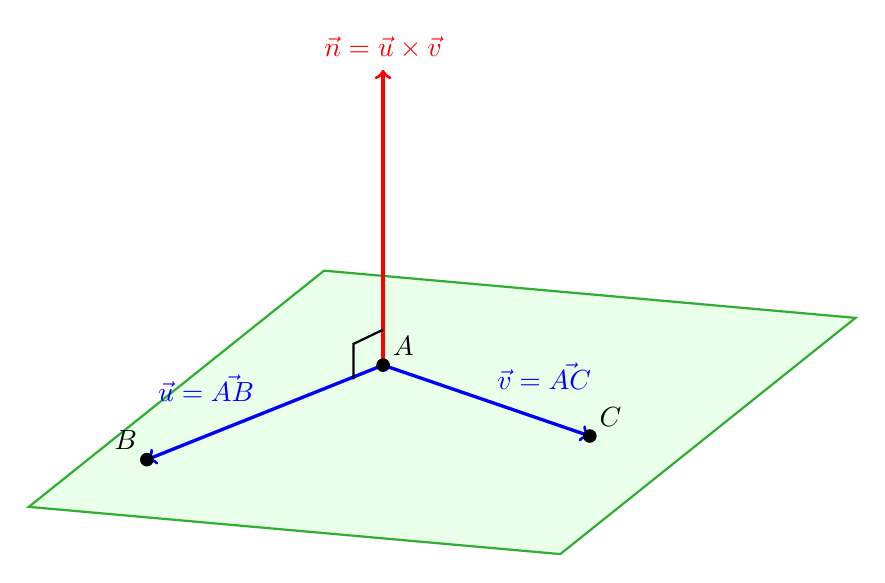
\begin{tikzpicture}[x={(-0.5cm,-0.4cm)}, y={(1cm,0cm)}, z={(0cm,1cm)}, scale=1.5]
    % Superficie del plano
    \filldraw[fill=green!10!white, draw=green!60!black, thick, opacity=0.8] 
        (-1,-1.5,0) -- (4,-1.5,0) -- (5,3.5,0) -- (0,3.5,0) -- cycle;
    
    % Puntos A, B y C
    \coordinate (A) at (1,0,0);
    \coordinate (B) at (3,-1,0);
    \coordinate (C) at (2.5,2.5,0);
    
    % Vectores directores u y v
    \draw[->, very thick, blue] (A) -- (B) node[midway, above left] {$\vec{u} = \vec{AB}$};
    \draw[->, very thick, blue] (A) -- (C) node[midway, above right] {$\vec{v} = \vec{AC}$};
    
    % Vector Normal (Producto Cruz)
    \draw[->, very thick, red] (A) -- ++(0,0,2.5) node[above] {$\vec{n} = \vec{u} \times \vec{v}$};
    
    % Perpendicularidad
    \draw[thick] (A) ++(0,0,0.3) -- ++(0.3,-0.1,0) -- ++(0,0,-0.3);
    
    % Puntos marcados
    \filldraw[black] (A) circle (1.5pt) node[above right] {$A$};
    \filldraw[black] (B) circle (1.5pt) node[above left] {$B$};
    \filldraw[black] (C) circle (1.5pt) node[above right] {$C$};
\end{tikzpicture}
\end{center}

\subsection{Intersecciones Espaciales}

\subsubsection{Intersección de un Plano con una Recta}

Sea la recta $\vec{r}(t) = \vec{r}_0 + t\vec{v}$ y el plano $ax + by + cz + d = 0$.\\

Expresando las coordenadas de la recta en su forma paramétrica: $x = x_0 + at$, $y = y_0 + bt$, $z = z_0 + ct$.

Sustituyendo estas expresiones en la ecuación del plano:
    $$ a(x_0 + v_1 t) + b(y_0 + v_2 t) + c(z_0 + v_3 t) + d = 0 $$

Despejando el parámetro $t$:
    $$ t = \frac{-(ax_0 + by_0 + cz_0 + d)}{av_1 + bv_2 + cv_3} = \frac{-(\vec{n} \cdot \vec{r}_0 + d)}{\vec{n} \cdot \vec{v}} $$

Si $\vec{n} \cdot \vec{v} = 0$, la recta es paralela al plano, por lo tanto, no hay intersección o está contenida en él. Si hay un valor finito de $t$, se sustituye en la ecuación de la recta para hallar el punto exacto.

\begin{center}
\shorthandoff{>}
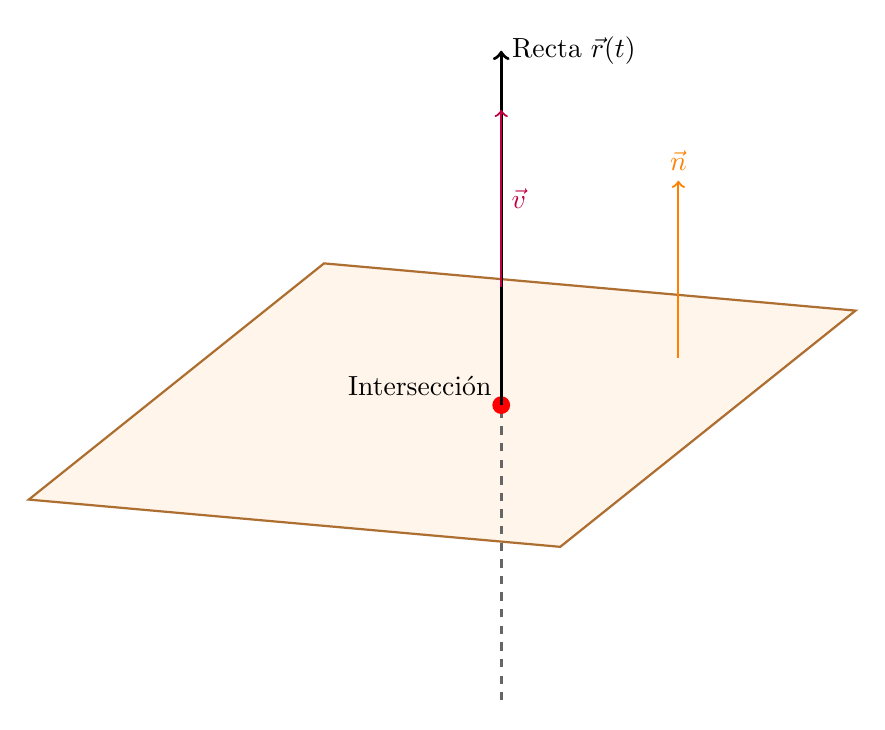
\begin{tikzpicture}[x={(-0.5cm,-0.4cm)}, y={(1cm,0cm)}, z={(0cm,1cm)}, scale=1.5]
    % Plano
    \filldraw[fill=orange!10!white, draw=orange!60!black, thick, opacity=0.8] 
        (-2,-2,0) -- (3,-2,0) -- (4,3,0) -- (-1,3,0) -- cycle;
    
    % Coordenadas de la recta
    \coordinate (L_start) at (1, 1, -2.5);
    \coordinate (L_int) at (1, 1, 0); % Punto de intersección
    \coordinate (L_end) at (1, 1, 3);
    
    % Recta debajo del plano (punteada para dar efecto de profundidad)
    \draw[dashed, very thick, black!60] (L_start) -- (L_int);
    
    % Punto de intersección
    \filldraw[red] (L_int) circle (2pt) node[above left, black] {Intersección};
    
    % Recta por encima del plano
    \draw[->, very thick, black] (L_int) -- (L_end) node[right] {Recta $\vec{r}(t)$};
    
    % Vector director de la recta
    \draw[->, thick, purple] (L_int) ++(0,0,1) -- ++(0,0,1.5) node[midway, right] {$\vec{v}$};
    
    % Vector normal del plano (como referencia visual)
    \draw[->, thick, orange] (0,2,0) -- (0,2,1.5) node[above] {$\vec{n}$};
\end{tikzpicture}
\end{center}

\subsubsection{Intersección entre dos Planos}

Dos planos no paralelos se intersectan siempre formando una línea recta. 

Para definir dicha recta $L$:
\begin{enumerate}
    \item La recta debe ser perpendicular a los dos vectores normales $\vec{n}_1$ y $\vec{n}_2$. Por lo tanto, su dirección es:
    $$ \vec{v}_L = \vec{n}_1 \times \vec{n}_2 $$
    \item Se resuelve el sistema de dos ecuaciones con tres incógnitas. Usualmente, se asigna un valor arbitrario a una variable y se resuelve el sistema de $2 \times 2$ resultante para $x$ e $y$ para encontrar un punto en común en ambos planos.
\end{enumerate}

\begin{center}
\shorthandoff{>}
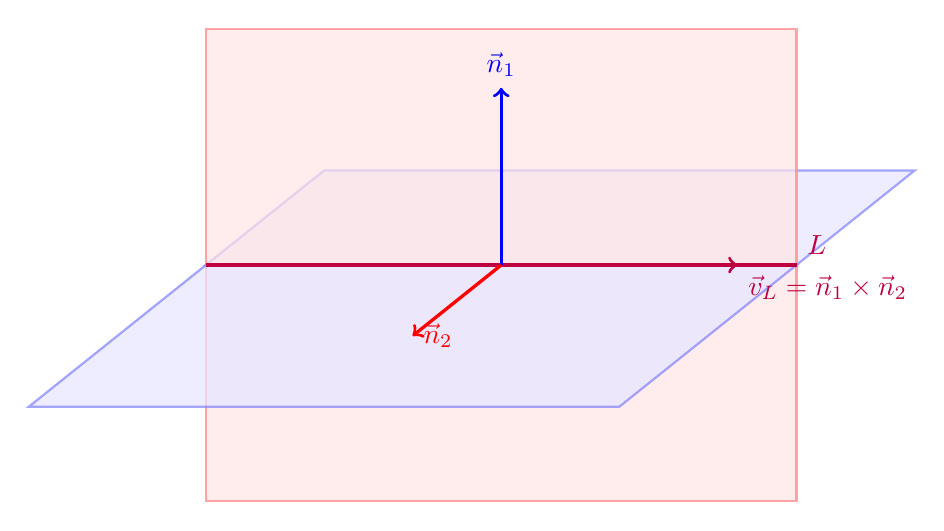
\begin{tikzpicture}[scale=1.5, x={(-0.5cm,-0.4cm)}, y={(1cm,0cm)}, z={(0cm,1cm)}]
    % Plano 1 (Horizontal, dibujado mitad atrás)
    \filldraw[fill=blue!10!white, draw=blue!50!white, thick, opacity=0.7] 
        (-2,-2,0) -- (0,-2,0) -- (0,3,0) -- (-2,3,0) -- cycle;
        
    % Plano 2 (Vertical-inclinado)
    \filldraw[fill=red!10!white, draw=red!50!white, thick, opacity=0.7] 
        (0,-2,-2) -- (0,3,-2) -- (0,3,2) -- (0,-2,2) -- cycle;
        
    % Plano 1 (Horizontal, dibujado mitad adelante para efecto 3D)
    \filldraw[fill=blue!10!white, draw=blue!50!white, thick, opacity=0.7] 
        (0,-2,0) -- (3,-2,0) -- (3,3,0) -- (0,3,0) -- cycle;

    % Línea de intersección
    \draw[very thick, purple] (0,-2,0) -- (0,3,0) node[above right] {$L$};
    
    % Vectores Normales
    \draw[->, very thick, blue] (0,0.5,0) -- (0,0.5,1.5) node[above] {$\vec{n}_1$};
    \draw[->, very thick, red] (0,0.5,0) -- (1.5,0.5,0) node[right] {$\vec{n}_2$};
    
    % Vector Director de la recta de intersección
    \draw[->, very thick, purple] (0,1.5,0) -- (0,2.5,0) node[below right] {$\vec{v}_L = \vec{n}_1 \times \vec{n}_2$};
\end{tikzpicture}
\end{center}

\subsection{Distancia de un Punto a un Plano}

Sea un punto exterior $S(x_1, y_1, z_1)$ y un plano definido por $ax + by + cz + d = 0$. La distancia mínima $D$ entre el punto y el plano es la longitud del segmento perpendicular desde $S$ hasta el plano.

Definase $P(x_0, y_0, z_0)$ como un punto cualquiera que pertenezca al plano. Se define el vector $\vec{PS} = (x_1-x_0, y_1-y_0, z_1-z_0)$.
La distancia $D$ es la magnitud de la proyección escalar de $\vec{PS}$ sobre el vector normal $\vec{n}$:
$$ D = |\text{proy}_{\vec{n}} \vec{PS}| = \frac{|\vec{PS} \cdot \vec{n}|}{\|\vec{n}\|} $$



Al desarrollar el producto punto en el numerador:
$$ \vec{PS} \cdot \vec{n} = a(x_1-x_0) + b(y_1-y_0) + c(z_1-z_0) = ax_1 + by_1 + cz_1 - (ax_0 + by_0 + cz_0) $$
Sustituyendo la condición del punto $P$ ($ax_0 + by_0 + cz_0 = -d$):
$$ \vec{PS} \cdot \vec{n} = ax_1 + by_1 + cz_1 - (-d) = ax_1 + by_1 + cz_1 + d $$

\begin{mydefinition}{Fórmula de Distancia Punto-Plano}
La distancia $D$ del punto $S(x_1, y_1, z_1)$ al plano $ax + by + cz + d = 0$ está dada por:
$$ D = \frac{|ax_1 + by_1 + cz_1 + d|}{\sqrt{a^2 + b^2 + c^2}} $$
\end{mydefinition}

\begin{center}
\shorthandoff{>}
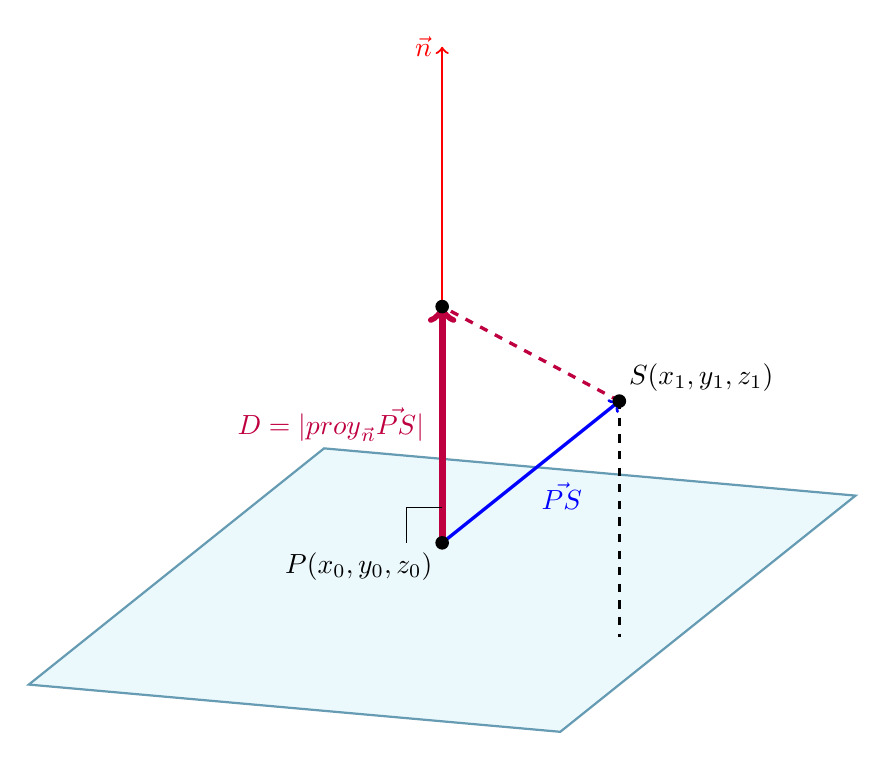
\begin{tikzpicture}[x={(-0.5cm,-0.4cm)}, y={(1cm,0cm)}, z={(0cm,1cm)}, scale=1.5]
    % Superficie del plano
    \filldraw[fill=cyan!10!white, draw=cyan!60!black, thick, opacity=0.8] 
        (-2,-2,0) -- (3,-2,0) -- (4,3,0) -- (-1,3,0) -- cycle;
        
    % Puntos clave
    \coordinate (P) at (0,0,0);     
    \coordinate (S) at (2, 2.5, 2); 
    \coordinate (ProjN) at (0, 0, 2); 
    \coordinate (Proj) at (2,2.5,0);
    
    \draw[->, thick, red] (P) -- (0,0,4.2) node[left] {$\vec{n}$};
    
    \draw[->, line width=2.5pt, purple] (P) -- (ProjN) node[midway, left=2pt] {$D = |\text{proy}_{\vec{n}}\vec{PS}|$};
    
    \draw[->, very thick, blue] (P) -- (S) node[midway, below right] {$\vec{PS}$};
    
    \draw[dashed, very thick, purple] (S) -- (ProjN);
    \draw[dashed, very thick, black] (S) -- (Proj);
    
    \draw (0, 0, 0.3) -- (0, -0.3, 0.3) -- (0, -0.3, 0);
    
    \filldraw[black] (P) circle (1.5pt) node[below left] {$P(x_0,y_0,z_0)$};
    \filldraw[black] (S) circle (1.5pt) node[above right] {$S(x_1,y_1,z_1)$};
    \filldraw[black] (ProjN) circle (1.5pt);
\end{tikzpicture}
\end{center}